% A skeleton file for producing Computer Engineering reports
% https://kgcoe-git.rit.edu/jgm6496/KGCOEReport_template

\documentclass[CMPE]{KGCOEReport}

% The following should be changed to represent your personal information
\newcommand{\classCode}{CMPE 160}  % 4 char code with number
\newcommand{\name}{Andrei Tumbar}
\newcommand{\LabSectionNum}{4}
\newcommand{\LabInstructor}{Mr.\ Byers}	% The slash is to tell LaTeX that the period is between words
												% not sentences so it spaces correctly. It won't appear in the
												% final pdf
\newcommand{\TAs}{Sam Myers \\ Kobe Balin \\ Georgi Thomas}
\newcommand{\LectureSectionNum}{1}
\newcommand{\LectureInstructor}{Mr.\ Cliver}
\newcommand{\exerciseNumber}{6}
\newcommand{\exerciseDescription}{Binary Addition and Subtraction Circuits}
\newcommand{\dateDone}{February 20th}
\newcommand{\dateSubmitted}{February 27th}

\graphicspath{{./lab6_media/}}

\usepackage{circuitikz}
\usepackage{tikz}
\usepackage{multirow}
\usepackage{titlesec}
\usepackage{float}
\usepackage{pgfplots, pgfplotstable}
\usepackage{lmodern}
\usepackage{siunitx}
\usepackage{subcaption}

\usepackage[usestackEOL]{stackengine}
\usepackage{scalerel}

\usepackage{kmap}
\usepackage[T1]{fontenc}

\usepackage{amsmath}

\def\lbar#1{\ThisStyle{%
  \setbox0=\hbox{$\SavedStyle#1$}%
  \stackengine{2.2\LMpt}{$\SavedStyle#1$}{\rule{\wd0}{0.1\LMpt}}{O}{c}{F}{F}{S}%
}}

\ctikzset{bipoles/not port/circle width=.4}
\ctikzset{tripoles/american and port/width=0.8}

\DeclareFontFamily{U}{mathx}{\hyphenchar\font45}
\DeclareFontShape{U}{mathx}{m}{n}{ <-> mathx10 }{}
\DeclareSymbolFont{mathx}{U}{mathx}{m}{n}
\DeclareFontSubstitution{U}{mathx}{m}{n}
\DeclareMathAccent{\widebar}{\mathalpha}{mathx}{"73}

\makeatletter
\newcommand{\cwidebar}[2][0]{{\mathpalette\@cwidebar{{#1}{#2}}}}
\newcommand{\@cwidebar}[2]{\@cwideb@r{#1}#2}
\newcommand{\@cwideb@r}[3]{%
  \sbox\z@{$\m@th\mkern-#2mu#3\mkern#2mu$}%
  \widebar{\box\z@}%
}
\makeatother

\begin{document}
\maketitle

\section*{Abstract}
In this laboratory exercise a binary adder/subtractor was implemented using the 2's complement implementation of subtraction. First a full adder was implemented by creating a Karnaugh Map and then reducing the boolean expression. A full adder's output consists of a sum and a carry which will go into the next full adder. K-Maps and boolean expressions were written for both. The circuits were created in Quartus and simulated in ModelSim. A VHDL test bench was provided for input signal control. Following the creation of a single full adder, a four-bit full adder was then given. By using a control signal and two four-bit binary numbers, an adder/subtractor was created in Quartus. Both the full adder and the 4-bit adder/subtractor was implemented on the breadboard. This exercise was successful in creating a circuit that adds and subtracts arbitrary inputs.

\section*{Design Methodology}

To first implement a full adder, a Karnaugh Map must be formed. Then, will the resultant boolean expression, a circuit diagram can be formed.

\subsection*{Full Adder}

Two Karnaugh Maps were created to implement both outputs of the adder. The letters $A$ and $B$ denote the two binary numbers being added while $C$ denote the carry in of the full adder.

\begin{figure}[h!]
	\begin{subfigure}{.5\textwidth}
		\centering
		\begin{Karnaugh24}
				\contingut{0,1,1,0,
						   1,0,0,1}
		   \implicant{4}{4}{blue}
		   \implicant{1}{1}{green}
		   \implicant{7}{7}{red}
		   \implicant{2}{2}{yellow}
		\end{Karnaugh24}
		\caption{K-Map of sum function.}
		\label{fig:sum}
	\end{subfigure}
	\begin{subfigure}{.5\textwidth}
		\centering
		\begin{Karnaugh24}
				\contingut{0,0,0,1,
						   0,1,1,1}
		   \implicant{5}{7}{blue}
		   \implicant{7}{6}{red}
		   \implicant{3}{7}{green}
		\end{Karnaugh24}
		\caption{K-Map of carry function.}
		\label{fig:carry}
	\end{subfigure}
	
	\caption{K-Maps for both outputs of the full adder.}
	\label{fig:kmap}
\end{figure}

None of the groups in Figure \ref{fig:sum} overlapped meaning that no boolean reduction from the k-map can be completed. In Figure \ref{fig:carry} three different groups are created. A min-term expression can be extracted from these k-maps. These terms can then be reduced to use fewer gates.

The letter $F$ will be used to express the full adder function. Therefore to distinguish each output $F_S$ will denote the sum and $F_C$ will denote the carry. $A$, $B$, and $C$ will be the inputs from the Karnaugh maps.

\begin{equation}
\label{eq:fs}
F_S = A\widebar{B}\widebar{C} + \widebar{A}\widebar{B}C + ABC + \widebar{A}B\widebar{C}
\end{equation}

\begin{equation}
\label{eq:fc}
F_C = AC + BC + AB = A(B + C) + BC
\end{equation}

All of the min-terms in the Figure \ref{fig:sum} were written as a boolean expression. Next, using the rules of boolean, $F_S$ (equation \ref{eq:fs}) can be simplified. Equation \ref{eq:fc} shows the min-terms of $F_C$ and a simple distributive simplification performed to reduce the total number of gates used.

\begin{align*}
    F_S &= \widebar{B}(A\widebar{C} + \widebar{A}C) + ABC + \widebar{A}B\widebar{C} && \text{Distributive property}\\
    &= \widebar{B}(A \oplus C) + ABC + \widebar{A}B\widebar{C} && \text{Definition of XOR}\\
    &= \widebar{B}(A \oplus C) + B(AC + \widebar{A}\widebar{C}) && \text{Distributive property}\\
    &= \widebar{B}(A \oplus C) + B(\lbar{\lbar{AC + \widebar{A}\widebar{C}}}) && \text{Double negation}\\
    &= \widebar{B}(A \oplus C) + B(\lbar{\cwidebar{AC} \cdot \cwidebar{\widebar{A}\widebar{C}}}) && \text{De-Morgan's Law}\\
    &= \widebar{B}(A \oplus C) + B(\lbar{(\widebar{A} + \widebar{C}) \cdot (A + C)}) && \text{De-Morgan's Law}\\
    &= \widebar{B}(A \oplus C) + B(\lbar{\widebar{A}A + \widebar{A}C + A\widebar{C} + \widebar{C}C}) && \text{Distributive property}\\
    &= \widebar{B}(A \oplus C) + B(\lbar{\widebar{A}C + A\widebar{C}}) && \text{Compliment Law}\\
    &= \widebar{B}(A \oplus C) + B(\lbar{A \oplus C}) && \text{Distributive property}\\
    &= B \oplus (A \oplus C) && \text{Definition of XOR} \\
    &= B \oplus A \oplus C && \text{Associative property} \\
    &= A \oplus B \oplus C && \text{Commutative property} \\
\end{align*}

Both of the functions are then implemented using AOI logic in Quartus.

\begin{figure}[h!]
	\centering
	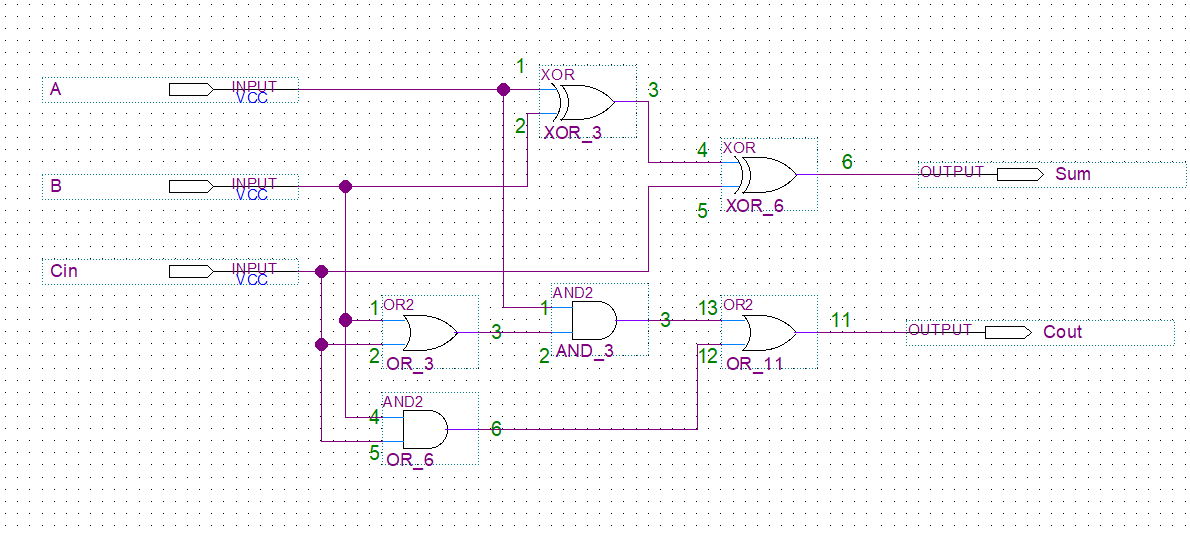
\includegraphics[height=6cm]{circuit}
	\caption{Circuit simulation using the test bench}
	\label{fig:fulladder}
\end{figure}

Figure \ref{fig:fulladder} is a circuit diagram of the three-input, four-output full adder using the boolean expressions previously derived.

\subsection*{4-bit Adder/Subtractor}

Adding binary numbers can be achieved by chaining multiple full-adders together can wiring the $C_{out}$ of one full-adder to the $C_{in}$ of the next adder. Subtraction can be thought of as adding a negative number. When a number is represented in 2's complement, adding negative numbers works just as their positive counterparts. A 2's complement number can be formed from its opposite by negating each bit and adding 1 to the result. Therefore subtraction can be done by inverting the inputs to each of the bits of one number and then setting the $C_{in}$ of the first adder to 1. By setting the carry to 1, we are effectively adding 1 to the summation of the first bit. However, merely adding an inverter would limit the circuit to only subtraction. The XOR gate solves this problem by acting as an inverter for the first input if the second input is 1 and a wire if the second input is 0. Therefore a control pin can be used to invert the inputs of one number and act as the $C_{in}$ for 4-bit adder.

\begin{figure}[h!]
	\centering
	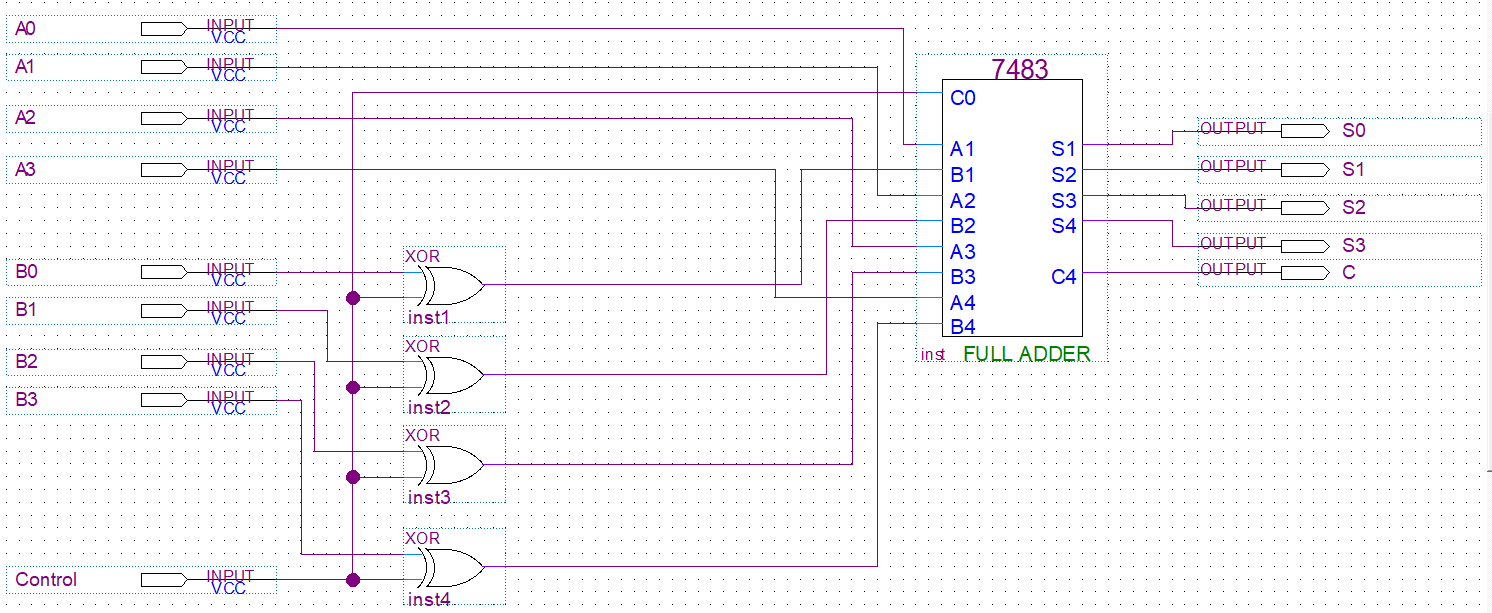
\includegraphics[width=\textwidth]{4-bit_full}
	\caption{4-bit full adder with subtraction control.}
	\label{fig:4bitadder}
\end{figure}

Figure \ref{fig:4bitadder} shows the Quartus diagram of the adder/subtractor. The two binary numbers $A$ and $B$ are represented with four input pins. $A0$ and $B0$ are the least significant bits (LSB). The inputs are feeding into a 74LS83 chip which consists of four fast-adders. The final input pin is labeled control. When set to \texttt{HIGH} the control pin will invert the signals for $B$. The control is also connected to $C0$ on the adder chip. This will add one as previously discussed. \\

The outputs $S0$ through $S4$ represent the bits on the output from the summation of the two input numbers. $C$ is the carry from the final adder inside the 74LS83 chip.

\section*{Results and Analysis}

\subsection*{1-bit full adder}

The single full-adder designed in the previous part was tested inside Multisim to verify the outputs. A VHDL test bench was provided to control the inputs $A$, $B$, and $C$.

\begin{figure}[h!]
	\centering
	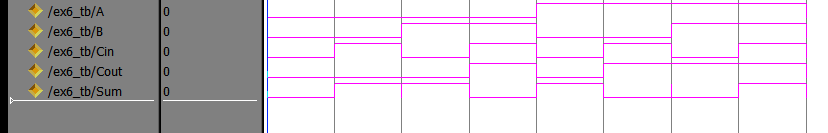
\includegraphics[width=\textwidth]{1-bit_full_vhdl}
	\caption{Simulation of full adder implementation.}
	\label{fig:simulation}
\end{figure}

Figure \ref{fig:simulation} shows the outputs of the sum and carry functions. The results match those in the Karnaugh Map in Figure \ref{fig:kmap}. This means that the circuit was implemented correctly.

\subsection*{4-bit adder/subtractor}

The circuit pictured in Figure \ref{fig:4bitadder} was constructed on a breadboard and then tested using a variety of input patterns.

\begin{table}[h]
\renewcommand{\arraystretch}{1.2}
\setlength{\tabcolsep}{12pt}
\caption{Four-bit binary addition}
\begin{center}
\begin{tabular}{|c|c||c|c||r|}
\hline
A3 A2 A1 A0 & B3 B2 B1 B0 & C4 & F3 F2 F1 F0 & $A + B = F$\\\hline
1 0 1 0 & 0 0 1 1 & 0 & 1 1 0 1 & $(-6) + (3) = -3$\\\hline
1 1 1 1 & 1 1 1 1 & 1 & 1 1 1 0 & $(-1) + (-1) = -2$\\\hline
1 1 1 1 & 0 1 1 0 & 1 & 0 1 0 1 & $(-1) + (6) = 5$\\\hline
0 1 1 1 & 0 0 1 1 & 0 & 1 0 1 0 & $(7) + (3) = -6$\\\hline
0 1 0 1 & 1 0 1 0 & 0 & 1 1 1 1 & $(-6) + (5) = -1$\\\hline
\end{tabular}
\end{center}
\label{tab:add}
\end{table}

\begin{table}[h!]
\renewcommand{\arraystretch}{1.2}
\setlength{\tabcolsep}{12pt}
\caption{Four-bit binary subtraction}
\begin{center}
\begin{tabular}{|c|c||c|c||r|}
\hline
A3 A2 A1 A0 & B3 B2 B1 B0 & C4 & F3 F2 F1 F0 & $A - B = F$\\\hline
1 0 1 0 & 0 0 1 1 & 1 & 0 1 1 1 & $(-6) - (3) = 7$\\\hline
1 1 1 1 & 1 1 1 1 & 1 & 0 0 0 0 & $(-1) - (-1) = 0$\\\hline
1 1 1 1 & 0 1 1 0 & 1 & 1 0 0 1 & $(-1) - (6) = -7$\\\hline
0 1 1 1 & 0 0 1 1 & 1 & 0 1 0 0 & $(7) - (3) = 4$\\\hline
0 1 0 1 & 1 0 1 0 & 0 & 1 0 1 1 & $(5) - (-6) = -5$\\\hline
\end{tabular}
\end{center}
\label{tab:sub}
\end{table}

Table \ref{tab:add} shows five examples of binary addition. All of the outputs correspond to those in decimal except for the fourth row. Here the output of $7 + 3$ turns out to be $-6$. This is because the $7$ is the maximum positive number a 4-bit 2's comp number can hold. This is because the first bit is for the sign therefore there are only 3-bits that can hold the number. When the addition overflows the number will wrap to the smallest negative value (-8). Rows 1 and 5 in Figure \ref{tab:sub} run in to the same problem.

\section*{Conclusion}

This exercise was implemented a full adder using simple logic gates. Then a 4-bit adder to create an adder/subtractor with 9-inputs and 5-outputs. A simulation of the full adder was performed in Multisim to verify the circuit against a Karnaugh Map. Both the full adder and the 4-bit adder/subtractor were constructed on a breadboard to test the signal outputs using LEDs. The exercise was successful in that the correct outputs were displayed given arbitrary inputs.

\section*{Questions}

\begin{enumerate}
  \item The simplest way to combine two full adders is to wire the $C_{out}$ of the LSB to the $C_{in}$ of the MSB.
  
  
  
\begin{figure}[htbp]
	\begin{center}
		\begin{circuitikz}
		
		\draw (0,0) node[dipchip,
			num pins=6,
			hide numbers, no topmark, external pins width=0.0](LSB){A0};
	
		\node [right, font=\tiny] at (LSB.bpin 1) {A0};
		\node [right, font=\tiny] at (LSB.bpin 2) {B0};
		\node [right, font=\tiny] at (LSB.bpin 3) {$C_{in}$};
		\node [left, font=\tiny]  at (LSB.bpin 6) {Sum};
		\node [left, font=\tiny]  at (LSB.bpin 4) {$C_{out}$};
		
		\draw (3,0) node[dipchip,
			num pins=6,
			hide numbers, no topmark, external pins width=0.0](MSB){A1};
	
		\node [right, font=\tiny] at (MSB.bpin 1) {A1};
		\node [right, font=\tiny] at (MSB.bpin 2) {B1};
		\node [right, font=\tiny] at (MSB.bpin 3) {$C_{in}$};
		\node [left, font=\tiny]  at (MSB.bpin 6) {Sum};
		\node [left, font=\tiny]  at (MSB.bpin 4) {$C_{out}$};
		
		\coordinate (start) at (0,-2);
		
		\draw (start) ++(0,0) coordinate(A0) node [below, font=\tiny]{A0};
		\draw (start) ++(1,0) coordinate(B0) node [below, font=\tiny]{B0};
		\draw (start) ++(2,0) coordinate(A1) node [below, font=\tiny]{A1};
		\draw (start) ++(3,0) coordinate(B1) node [below, font=\tiny]{B1};
		
		\draw (A0) |- ++(-1.5,0.5) |- (LSB.pin 1);
		\draw (B0) |- ++(-2.25,0.75) |- (LSB.pin 2);
		\draw (A1) |- ++(-0.5, 0.5) |- (MSB.pin 1);
		\draw (B1) |- ++(-1.25,0.75) |- (MSB.pin 2);
		
		\draw (LSB.pin 4) -- (MSB.pin 3);
		\draw (LSB.pin 6) -| ++(0.5,1) node[above, font=\tiny]{S0};
		\draw (MSB.pin 6) -| ++(0.5,1) node[above, font=\tiny]{S1};
		
		\draw (LSB.pin 3) -- ++(-1.5,0) node[ground]{};
		\draw (MSB.pin 4) -- ++(0.5,0) node[right, font=\tiny]{$C_{out}$};
		
		\end{circuitikz}
	\end{center}
	\caption{Two bit ripple-carry adder.}
	\label{fig:ripple}
\end{figure}

Figure \ref{fig:ripple} shows two full adders chained together by feeding the $C_{out}$ of the first into the $C_{in}$ of the second. The $C_{in}$ of the LSB is connected to ground or 0 because there is no previous bit to carry from.

  \item Design a two level NOR-NOR implementation of $F_{POS}$.
  
\begin{figure}[htbp]
	\centering
	%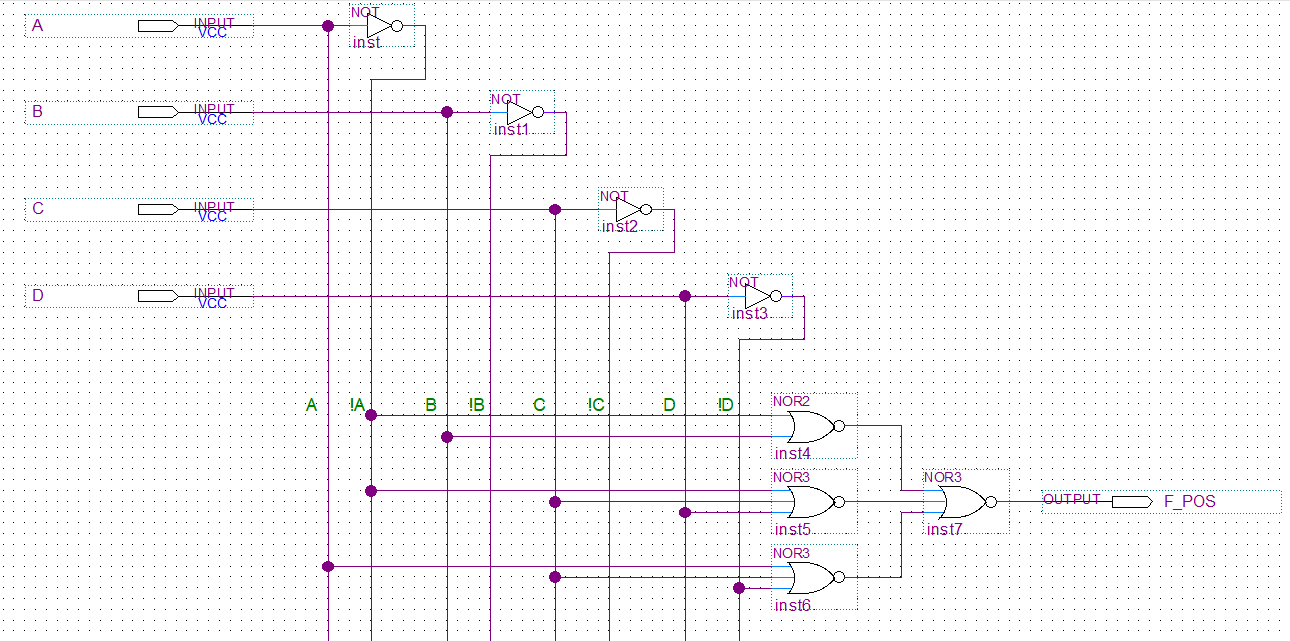
\includegraphics[height=7.5cm]{nor-nor}
	\caption{Two level NOR-NOR implementation of $F_{POS}$}
	\label{fig:nor-nor}
\end{figure}
\end{enumerate}

\end{document}
